\subsection{プロトコル階層とサービスモデル}

\subsubsection{階層化アーキテクチャ}

インターネットは極めて複雑なシステム
\begin{itemize}
  \item[] プロトコルならびに、それを動作させるハードウェア、ソフトウェアを階層化して設計
  \begin{itemize}
    \item[$\Rightarrow$] ネットワーク設計の複雑さを軽減し、各構成要素間の役割や関係を明確にする
    \item[] \textcolor{cyan}{モジュール化、個別に設計}
  \end{itemize}
\end{itemize}

各プロトコルはある一つの階層(layer)に属する
\begin{itemize}
  \item[] 第n層のプロトコルは第n層同士でメッセージを交換
  \begin{itemize}
    \item[] 第n層のプロトコルデータユニット(n-PDU): 第n層で交換されるメッセージ
  \end{itemize}
\end{itemize}

\begin{itemize}
  \item プロトコルスタック(protocol stack): これらのプロトコルが構成する階層全体
  \begin{itemize}
    \item[$\cdot$] OSI参照モデル(Open System Interconnection Refference Model): 7層構造
    \item[$\cdot$] インターネット(TCP/IP): 5層構造
  \end{itemize}
\end{itemize}

\begin{figure}[h]
  \centering
  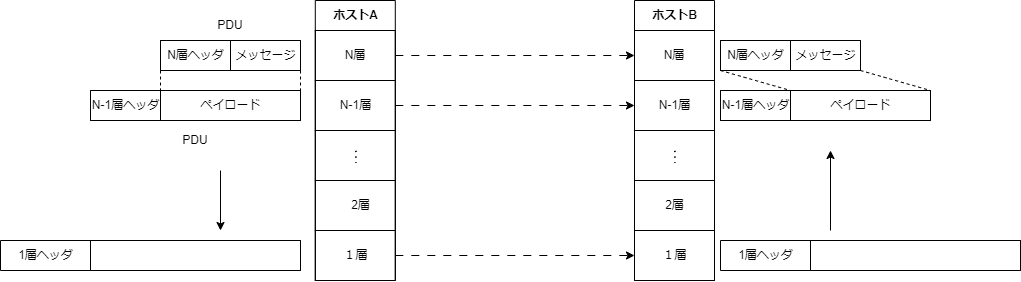
\includegraphics[width=0.8\linewidth]{image/npu.png}
\end{figure}


ホストAの第n層がホストBの第 n 層にn-PDUを送信
\begin{enumerate}
  \item ホストAの第n層がホストBの第 $n-1$ 層にn-PDUを渡し、ホストBの第n層への送信を依頼
  \item 第n層は第 $n-1$ 層のサービスを受ける  (第 $n-1$ 層は第n層にサービスを提供)
  \item 第n層は第 $n-1$ 層がどのようにサービスを実現しているかを意識しない
  \begin{itemize}
    \item[$\Rightarrow$] 層間のインターフェースが定義されていれば差し替え可能
    \item[] \textcolor{cyan}{抽象メソッドみたい}
  \end{itemize}
  \item[] \textcolor{cyan}{層が深くなるにつれ、誤り訂正などの処理が行われる}
\end{enumerate}


$\cdot$ プロトコル階層化の欠点
\begin{itemize}
  \item 同じ機能を複数の層が持つ場合がある (誤り制御など)
  \begin{itemize}
    \item[] \textcolor{cyan}{データ量的に無駄}
  \end{itemize}
  \item 上位層は下位層の情報を利用できない (柔軟性の欠如)
\end{itemize}


\newpage
\subsubsection{インターネットプロトコル階層}

\begin{table}[h]
  \centering
  \caption{}
  \label{tab:}
  \begin{tabular}{c|c|c}
    && PDUの呼び方\\\hline
    Layer 5 & アプリケーション & メッセージ \\
    Layer 4 & トランスポート & セグメント\\
    Layer 3 & ネットワーク データグラム(パケット)\\
    Layer 2 & データリンク & フレーム\\
    Layer 1 & 物理 & 1-PDU\\\hline
  \end{tabular}
\end{table}

\begin{itemize}
  \item アプリケーション層\\
    \underline{ネットワークアプリケーションをサポート}
  \begin{itemize}
    \item[例)] HTTP: web
    \item[] SMTP: 電子メール
    \item[] FTP: ファイル転送
  \end{itemize}
  \item トランスポート層\\
    \underline{アプリケーションプロセス間}のメッセージ転送サービスで提供
  \begin{itemize}
    \item TCP: 高信頼データ転送、フロー制御、輻輳制御
    \item UDP: コネクションレス型サービス
  \end{itemize}
  \item ネットワーク層\\
    始点・終点ホスト間でデータグラムの転送を行うIP・インターネットの3層プロトコル (IP層ともいう)
  \begin{itemize}
    \item[] IPデータグラムの定義と、それに基づくエンドシステムやルータの動作を規定
    \item ルーチングプロトコル:\\
      始点ホストから終点ホストまでの経路を設定\\
      複数のプロトコルが存在
    \end{itemize}
  \item データリンク層\\
    \underline{ノード間の1ホップ} の通信を担う
  \begin{itemize}
    \item[例)] Wi-Fi, イーサネット(有限LAN)など
  \end{itemize}
  \item 物理層
  \begin{itemize}
    \item フレーム内の各ビットを伝送
    \item \begin{tabbing}
      物理メディア: \=より対線、同軸ケーブル\\
      \>光ファイバ、無線など
    \end{tabbing}
  \end{itemize}
\end{itemize}

ネットワークエンティティ

\indent\indent ネットワークの構成要素(エンドシステムと中継器)
\begin{itemize}
  \item \begin{tabbing}
    中継器: \=ルータ(3層まで)\\
    \>ブリッジ、スイッチ(2層まで)
  \end{tabbing}
  \item エンドシステム: 5層すべて
\end{itemize}
